% !TEX TS-program = pdflatex
% !TEX encoding = UTF-8 Unicode

% This is a simple template for a LaTeX document using the "article" class.
% See "book", "report", "letter" for other types of document.

\documentclass[12pt]{article} % use larger type; default would be 10pt

\usepackage[utf8]{inputenc} % set input encoding (not needed with XeLaTeX)

%%% Examples of Article customizations
% These packages are optional, depending whether you want the features they provide.
% See the LaTeX Companion or other references for full information.

%%% PAGE DIMENSIONS
\usepackage{geometry} % to change the page dimensions
\geometry{a4paper} % or letterpaper (US) or a5paper or....
% \geometry{margin=2in} % for example, change the margins to 2 inches all round
% \geometry{landscape} % set up the page for landscape
%   read geometry.pdf for detailed page layout information

\usepackage{graphicx} % support the \includegraphics command and options

% \usepackage[parfill]{parskip} % Activate to begin paragraphs with an empty line rather than an indent

%%% PACKAGES
\usepackage{booktabs} % for much better looking tables
\usepackage{array} % for better arrays (eg matrices) in maths
\usepackage{paralist} % very flexible & customisable lists (eg. enumerate/itemize, etc.)
\usepackage{verbatim} % adds environment for commenting out blocks of text & for better verbatim
\usepackage{subfig} % make it possible to include more than one captioned figure/table in a single float
\usepackage{graphicx}
\usepackage[colorlinks, urlcolor=cyan, citecolor=red]{hyperref}
% These packages are all incorporated in the memoir class to one degree or another...

%%% HEADERS & FOOTERS
\usepackage{fancyhdr} % This should be set AFTER setting up the page geometry
\pagestyle{fancy} % options: empty , plain , fancy
\renewcommand{\headrulewidth}{0pt} % customise the layout...
\lhead{}\chead{}\rhead{}
\lfoot{}\cfoot{\thepage}\rfoot{}

%%% SECTION TITLE APPEARANCE
\usepackage{sectsty}

\usepackage{enumitem}

%%% ToC (table of contents) APPEARANCE
\usepackage[nottoc,notlof,notlot]{tocbibind} % Put the bibliography in the ToC
\usepackage[titles,subfigure]{tocloft} % Alter the style of the Table of Contents
\usepackage{dirtree}
\usepackage{authblk}
\renewcommand{\cftsecfont}{\rmfamily\mdseries\upshape}
\renewcommand{\cftsecpagefont}{\rmfamily\mdseries\upshape} % No bold!

%%% END Article customizations

%%% The "real" document content comes below...

\title{OCR Handwriting Project Outline}
\author{Matthew Mulhall}
\affil{matthew.l.mulhall@uconn.edu}
%\date{} % Activate to display a given date or no date (if empty),
         % otherwise the current date is printed 

\begin{document}
\maketitle

\section{May 14, 2019}
\subsection{Summary of Design Decisions}

The project will follow an abstraction based design: letters, words, lines, and entire documents. Every document can be broken down into these respective groups of abstraction.

\begin{enumerate}[label = (\roman*)]
\item An entire document.
\item A collection of lines in a document.
\item A collection of words that are consecutively placed on each line.
\item Single characters that make up the words.
\end{enumerate}
It can be seen that each level abstraction relies on the previous, going all the way down to the individual letters that are on the document. Given the nature of that abstraction Dr. Johnson suggested we start from the ground up, meaning first we will be building the data set for letters, and training a model to recognize other letters of similar (1800's English) style. Our current priority is to build this large data set of characters for our neural network to pull from. After this set is built up we will work on figuring out the optimal design of our model and start to train it. After this section is completed we will have a network that can identify individual characters. From this base level we will then work on the next level of abstraction, that will be able to identify the words in a line. The project will follow a similar style of abstraction based progress until we can use every level to read an entire document.

\subsection{Some specifics}
We currently have 7 documents that have been allocated for our project. The first 4 will be used to create the data set of images. On top of simple screenshots, we will also employ GPUs to transform the images to get the most mileage out of each photo. The last 3 will be later allocated into development and strict testing sets. These will be allocated as the training set is developed.
\subsection{Description of file system}
\dirtree{%
.1 OCR-Handwriting .
.2 bin .
.3 src .
.3 data.
.4 char .
.5 ascii lower .
.6 a to z.
.5 ascii upper.
.6 A to Z.
.5 ascii number.
.6 0 to 9 .
.5 compound .
.5 punctuation .
.4 documents .
.5 Training Set.
.2 documentation .
.3 Project Log.
.3 Completion Log.
.2 utilities .
}
\begin{enumerate}[label = (\roman*)]
\item Bin contains all of the 'raw' data such as images, and documents where the images come from. Each sub directory is ordered.
\item The section 'compound' has been added due to the nature of John Quincy Adams handwriting. There are several small phrases like 'Mr' and 'Dr' that appear more as one character than 2. This is why it is denoted as 'compound', meaning more than one letter interpreted as a single unit.
\item Documentation contains this document, as well as any other documents that are needed to explain the project.
\item Utilities contains all scripts, programs, or software that we use as a supplement in order to complete the project.
\end{enumerate}

\subsection{Software Information}
\begin{enumerate}[label = (\roman*)]
\item Python 3.7.3
\item Github
\item \textbf{Packages:}
\item Keras
\item Tensorflow/Tensorflow-gpu
\item NumPY
\item cv2 (OpenCV)
\item imutils
\item GraphViz
\item Matplotlib
\item PyDot
\end{enumerate}

\subsection{Significant Developments}
\subsubsection{May 14, 2019}
Total images taken: 296\newline
\noindent\makebox[\linewidth]{\rule{15cm}{0.4pt}}
Matt created a python script that renames the pictures in the subdirectories according to a naming scheme, this allows for saving files without having to worry about typing the name into the save box. Doing this means the whole process takes ~10x less time. When taking photos one can either: focus on a letter saving several in a certain directory (fastest), or save all photos to a "dump" folder and place them afterwards in their correct directory.
\subsubsection{May 15, 2019}
Letters completed: 'a' , 'e' . \newline
Total images taken: 2,075 \newline
\noindent\makebox[\linewidth]{\rule{15cm}{0.4pt}}
\large{Process for quickest imaging (Modified 5/21):}
\begin{enumerate}[label = (\roman*)]
\item Pick a letter that has a lower than needed sample size ( < 500).
\item Using Lightshot, take a screenshot of a letter, and click the save button. Navigate to the respective directory and save.
\item For all subsequent letters, take the photo and use shortcut CTRL-S and it will auto-save to the same directory.
\item After you find as many as you can on the page, or several pages, move on to the next page.
\item After around 125-150 letters from a given set of pages, go onto another set of pages.
\item Before pushing to git, run the renameUtilityScript.py file which will rename all of the files to the appropriate schema.
\end{enumerate}

\subsection{May 16, 2019}
Letters completed: 'b'.\newline
Total images taken:  864\newline
\noindent\makebox[\linewidth]{\rule{15cm}{0.4pt}}
\begin{enumerate}[label = (\roman*)]
\item Made changes to the script so that it can be run on any machine without needing to edit the path in the file. If anybody wants to run it, python must be installed and they can either manually run it or write a bat file. There is a provided bat file skeleton, all that needs to be added is the path to the .py utility, and it can be run from anywhere.

\end{enumerate}

\subsection{May 21, 2019}
Letters completed: 'c', 'd', 'i', 'f', 'g', 'h'\newline
Total images taken: 3,054\newline
\noindent\makebox[\linewidth]{\rule{15cm}{0.4pt}}
\begin{enumerate}[label = (\roman*)]
\item Purchased the font "Old Man Eloquent" that we will use to diversify our samples. The current plan is to photograph the font in various contexts and use CUDA to transform the images to extract a large amount of diverse images from one example.
\item Mike and Matt had a conversation outlining the plan for hardware to be able to transform images. Once the types of image transformations are chosen, Matt will create software that will be able to be used without programming experience.
\item Matt suggested using an image normalization algorithm to give each image the same scale. It would involve locating the global min and max for width and height, and setting each photo to those dimensions. This could be important for making sure the network does not pick up on unintended scale related differences between letters.
\end{enumerate}

\subsection{May 22, 2019}
Letters completed: 'j', 'l', 'm', 'n'\newline
Total images taken: 1,928 \newline
\noindent\makebox[\linewidth]{\rule{15cm}{0.4pt}}
\begin{enumerate}[label = (\roman*)]
\item Matt created a completion log complete with all characters so that we can more easily keep track of completed characters.
\end{enumerate}

\subsection{May 23, 2019}
Letters completed: 'k', 'o', 'p'\newline
Total images taken:1,004\newline
\noindent\makebox[\linewidth]{\rule{15cm}{0.4pt}}
\begin{enumerate}[label = (\roman*)]
\item No important developments today. Good progress on imaging.
\end{enumerate}

\subsection{May 28, 2019}
Letters completed: 'q', 'r', 's', 't', 'u'\newline
Total images taken: 2,244 \newline
\noindent\makebox[\linewidth]{\rule{15cm}{0.4pt}}
\begin{enumerate}[label = (\roman*)]
\item Today we completed 5 characters towards the end of the alphabet. I have high confidence that by tomorrow we will complete all lowercase imaging. This means we are slightly under halfway to completing the data set
\item Another important development is that we passed 10,000 images in just 7 working days, a great achievement. We are currently working with: \bf{11,465} images.
\end{enumerate}

\subsection{May 29, 2019}
Letters completed: 'v', 'w', 'x', 'y', 'z'\newline
Total images taken: 1,924 \newline
\noindent\makebox[\linewidth]{\rule{15cm}{0.4pt}}
\begin{enumerate}[label = (\roman*)]
\item Today I completed 5 characters. Additionally, with the completion of 'z' the entire lowercase alphabet has been concluded. I would venture to say we are likely half way currently. Although there are more than just the upper-case section left, those are far less common and hence will include fewer screenshots.
\end{enumerate}

\subsection{May 30, 2019}
Total images taken: 1,001\newline
\noindent\makebox[\linewidth]{\rule{15cm}{0.4pt}}
\begin{enumerate}[label = (\roman*)]
\item Today I worked from home, the log is being updated retroactively.
\item The most important development from the day was a change in the way we collect screenshots for the upper case characters. Rather than picking a character and moving through each page for that character, for upper case (or generally less frequent sets of multiple characters) find all examples on the page and screenshot them. After this, move onto the next page.
\item Because the amount of upper case characters is far lower than lower case letters, we are just taking as many samples as we can get. Therefore there will be no more "letters completed." Upper case letters will be completed when all examples of them are recorded
\item Finished up to page 17 of DJQA 1829-02.
\end{enumerate}

\subsection{June 4th, 2019}
Total images taken: 1,495 \newline
\noindent\makebox[\linewidth]{\rule{15cm}{0.4pt}}
\begin{enumerate}[label = (\roman*)]
\item Today was a standard day, continued to image the upper case letters.
\item There was quite a lot of progress in terms of images taken as well as total traversal of the data set. We are almost half way through the data for upper case letters. This puts us in a great position, well over half way done with overall imaging.
\item Finished up to page 16 of DJQA 1829-03.
\end{enumerate}

\subsection{June 5th, 2019}
Total images taken: 1,247 \newline
\noindent\makebox[\linewidth]{\rule{15cm}{0.4pt}}
\begin{enumerate}[label = (\roman*)]
\item Not many important developments today, the only noticable change would be that as I have progressed, the density of upper case characters has seemed to dwindle, as can bee seen from the total for today.
\item Finished up to  DJQA 1829-04 section 17. Meaning we got just over 30 pages of material today, exactly the same as the previous 2 days of upper case imaging.
\end{enumerate}

\subsection{June 6th, 2019}
Total images taken: 936 \newline
\noindent\makebox[\linewidth]{\rule{15cm}{0.4pt}}
\begin{enumerate}[label = (\roman*)]
\item Completed up to DJQA 1829-05 section 19. On the road to complete upper case before lunch of the next work day.
\end{enumerate}

\subsection{June 11th, 2019}
Letters Completed: All capital letters besides 'O', 'L', 'X', 'Z'.\newline
Total images taken: 1,077 \newline
\noindent\makebox[\linewidth]{\rule{15cm}{0.4pt}}
\begin{enumerate}[label = (\roman*)]
\item Capital letters are virtually completed, all that is left is specfic imaging to expand the sets of several select capital letters.
\item Imaging has moved onto compound letters, completed through DJQA 1829-03 Section 20.
\end{enumerate}

\subsection{June 12th, 2019}
Letters Completed: 'Mrs', 'Mr', 'Dr', 'ss' \newline
Total images taken: 750 \newline
\noindent\makebox[\linewidth]{\rule{15cm}{0.4pt}}
\begin{enumerate}[label = (\roman*)]
\item Completed all compound letters.
\item After completing compound letters, we moved onto completion of imaging the numbers.
\item Imaging of numbers reached DJQA 1829-03 section 24.
\item Also did a lot of reading that is necessary for the continuation of the project.
\end{enumerate}

\subsection{June 13th, 2019}
Total images taken: ~750 \newline
\noindent\makebox[\linewidth]{\rule{15cm}{0.4pt}}
\begin{enumerate}[label = (\roman*)]
\item Continued imaging of numbers for numbers, currently on DJQA 1829-04 section 19.
\end{enumerate}

\subsection{June 18th, 2019}
Letters Completed: ':', comma, period, question mark, exclamation mark.\newline
Total images taken: ~800 \newline
\noindent\makebox[\linewidth]{\rule{15cm}{0.4pt}}
\begin{enumerate}[label = (\roman*)]
\item Significant imaging of the punctuation set.
\item The last 2-3 hours were spent on the first iteration of proof of concept.
\item This proof of concept will focus on making a convnet that properly identifies 4 of our letters with using minimal data altercations. After this we will move to iteration 2 where we simply alter the data. 
\item After 2 we will most likely open up to more letters and continually scale and test the software.
\item Phase 1 of the testing was completed. With a data set totaling 2,000 images in 4 categories (namely 'a', 'b', 'c', 'd') Matt constructed a convolutional
neural network that has a peak of 94.69\% validation accuracy. Note, the network did not use image preproccesing to change the size of the dataset, which will be used in test 2.
\item The network form that was used in this exercise was as follows:
\item Model: Sequential
\item Layer 1: Convolutional 2D
\item Layer 2: Max Pooling 2D
\item Layer 3: Convolutional 2D
\item Layer 4: Max Pooling 2D
\item Layer 5: Convolutional 2D
\item Layer 6: Max Pooling 2D
\item Layer 7: Convolutional 2D
\item Layer 8: Max Pooling 2D
\item Layer 9: Flatten
\item Layer 10: Dense (512)
\item Layer 11: Dense(4 - categories)
\item Below is an image that depicts the 'learning' of the model from test 1.
\item 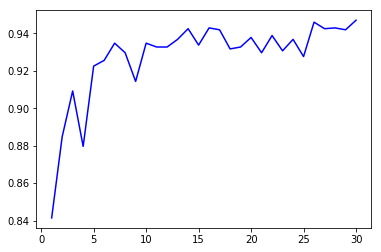
\includegraphics{convnet-test-1-val-acc}
\end{enumerate}

\subsection{June 19th, 2019}
\noindent\makebox[\linewidth]{\rule{15cm}{0.4pt}}
\begin{enumerate}[label = (\roman*)]
\item Today we began with phase two of the small set convnet. The changes will be as follows:\newline
 Steps per epoch up to 100, data augmentation (specifics provided in the code).
\item We completed all images today. The total count being 21,515 images. There are still some select images that I believe we will need to address, but this will happen as we continue our push forward in testing.
\item After completing the training of the new neural network that used augmentation we got the following results:
\item 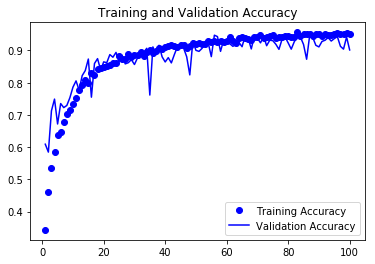
\includegraphics{convnet-test-2-val-acc}
\item As we can see, the tests did well to limit overfitting. However, further tuning is required to get our percentage even higher. Currently it lags at around 96\%
\item Today I created several important scripts for the project. The first is a utility to automate the entire prediction process of any model. In this file you give a path to an image and the program will predict, and create an image with text that displays the guess and its percentage certainty.
\item 
\includegraphics{This_is_d1}
\item This image shows an example of our second network trained with augmentation predicting a letter 'd'. The catch is, this was written by a different author than our training set!
\item The second script was a utility for moving through directories and placing photos in respective test/train/validation directories. This is much easier for med-large sets, rather than placing each image manually.
\end{enumerate}

\subsection{June 20th, 2019}
\noindent\makebox[\linewidth]{\rule{15cm}{0.4pt}}
\begin{enumerate}[label = (\roman*)]
\item Today I was able to do several things, first and foremost get better plots of the smallset test \#2.
\item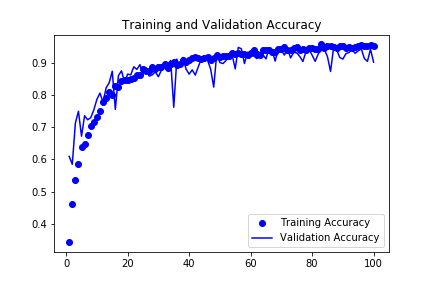
\includegraphics{train-vs-val-acc-small2}\newline 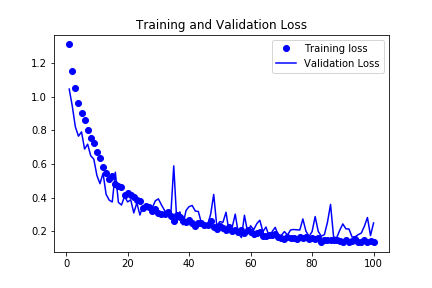
\includegraphics{train-vs-val-loss-small2}
\item As we can see from testing, this second network design, which includes augmentation, has far less over-fitting. This was to be expected, but the results are quite impressive. I suggest that for this second small set model we try varying epochs, and new layers.
\item Secondly I was able to finish the training of the med-set network, which did not turn out as we would have hoped. But not to be cynical, we will be able to fine tune this.
\item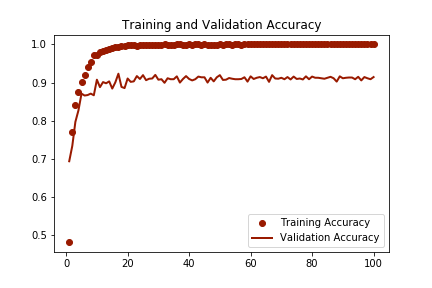
\includegraphics{train-vs-val-acc-med-1}\newline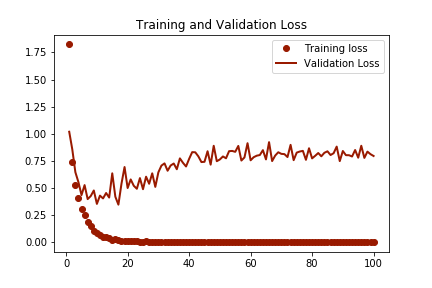
\includegraphics{train-vs-val-loss-med-1}
\item Although, on first glance, it appears that the validation accuracy was pretty good (although heavily over-fitted), yet the loss remained above 75\% for the duration of the training. I think that this means a few things, firstly we need to make the network deeper and use more advanced \textbf{layer techniques}. Secondly, adding image augmentation will certainly take a lot of that loss, and over-fitting away. These augmentations to the model will happen next Tuesday.
\end{enumerate}

\subsection{June 25th, 2019}
\noindent\makebox[\linewidth]{\rule{15cm}{0.4pt}}
\begin{enumerate}[label = (\roman*)]
\item Based on the poor showing of the previous model, to start the day I will try and modify it in a second medium test. This test will aim to bring the loss as low as possible.
\item Rather than continually attempting to adjust layers, I believe it would be intelligent to do the changes in batches and closely analyze the difference between each method. First we are adding data augmentation to the second test. After, we will move onto layer changes.
\item \textbf{Today I switched work stations to a computer with a GTX 1080, because of this, training time has decreased by 90\%}.
\item The following is the model design used in test 'medset-2', this model included augmented training images, defined by the parameters available on \href{https://github.com/mattlm0831/OCR-Handwriting/blob/master/bin/src/testing/convnet-medset-ocr-test2/convnet-medset-ocr-test2.py}{github}.
\item 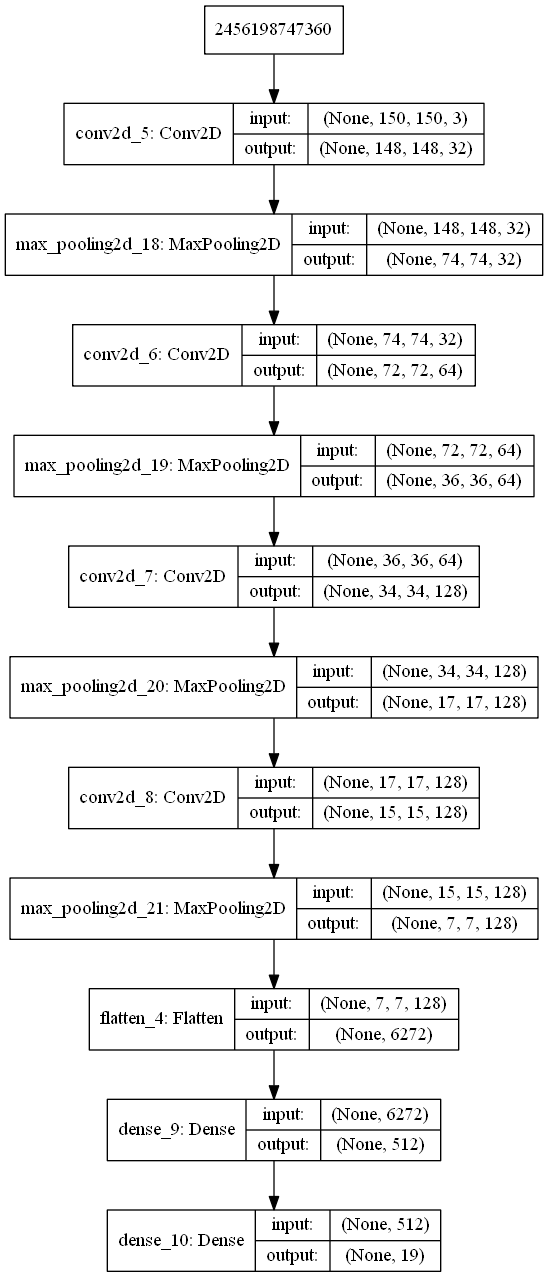
\includegraphics[height = 200mm, scale=.5]{model-medset2}
\item This model performed much better than the previous iteration due to augmentation. Albeit, still below our goals. The following graphics show that this model did much better dealing with overfitting:
\item 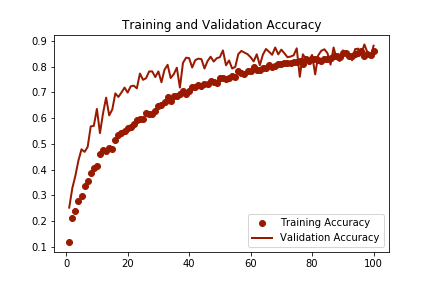
\includegraphics{train-vs-val-acc-medset2}
\item 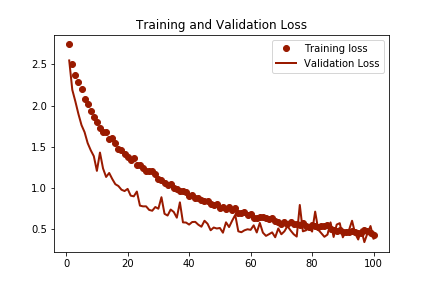
\includegraphics{train-vs-val-loss-medset2}
\item Some other important takeaways: Loss was kept far lower, decreased by 30\%\textsuperscript{+} relative to the previous test. Accuracy remained lower than previous attempts at 85\%, but in this context the lower accuracy is not a negative as it coincides with a falling loss value.
\item After feeling confident about the network structure in test 'medset-2' I continued onto test 'medset-3' to try and further the progress. The only difference for this test (medset-3) was doubling the epochs. I decided to make this choice because the network seemed to be continually improving, rather than reaching a plateu before 100 epochs. Continuing the training further has seemed to do a great deal of relative improvement on both loss and accuracy. The next test 'medset-4', will have to focus on continuing with this and perhaps extending even further if a plateu is not reached in the previous test.
\item Although the results are not perfect at the moment, in a mere day we have been able to take loss from .7 in medset1 to ~.28 in medset3.
\item As can be seen from the two following graphs, increasing epochs did translate to an increase in accuracy and decrease in loss (~90\% and ~28\% respectively). This bodes well for the future, we can use this to further explore techniques of training as a road to better results as well as hyper parameters.
\item 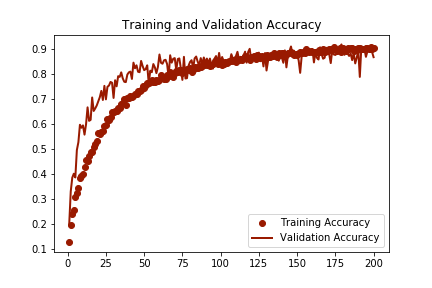
\includegraphics{train-vs-val-acc-medset3}
\item 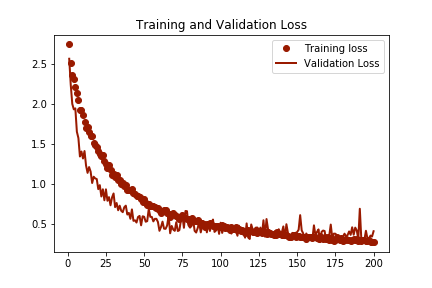
\includegraphics{train-vs-val-loss-medset3}
\end{enumerate}

\subsection{June 26th, 2019}
\noindent\makebox[\linewidth]{\rule{15cm}{0.4pt}}
\begin{enumerate}[label = (\roman*)]
\item Today I decided to train another model on the medium test set. This model will have several differences and similarities. It will be trained longer (250 epochs), have 64 for batch size, and will also have two dropout layers added. This model, denoted as medset4, will have the following form:
\item 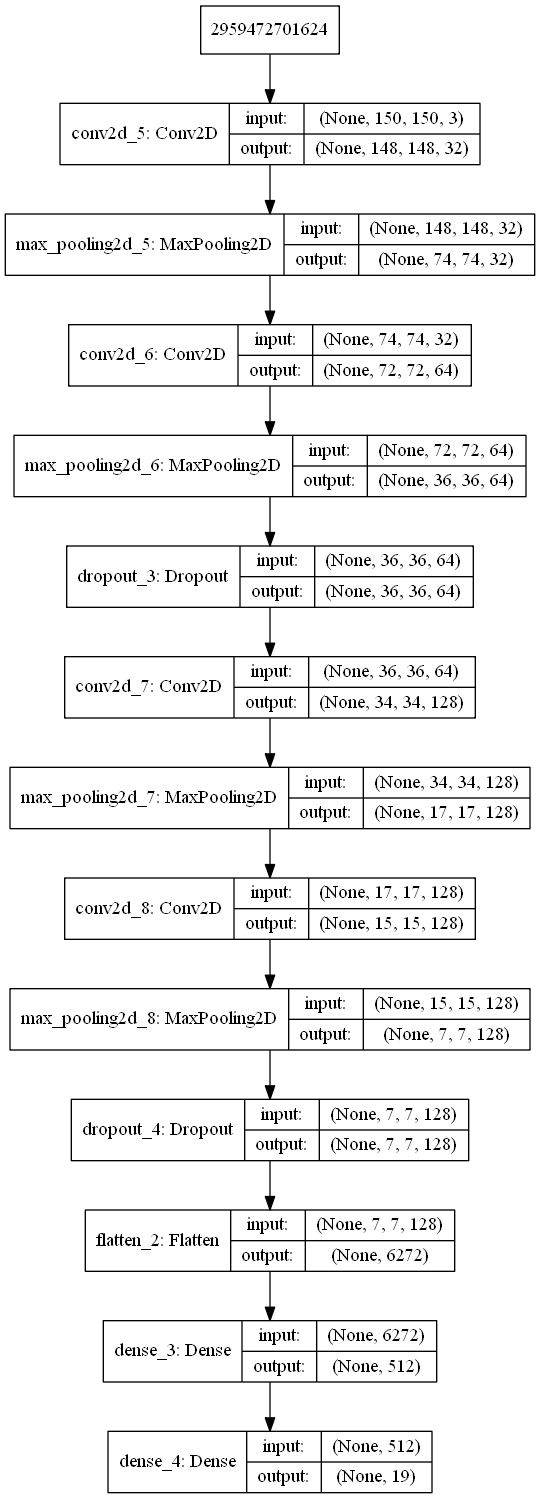
\includegraphics[height = 200mm, scale=.5]{model-medset4}
\item This model performed very well. Pushing our loss further to a cool 21\% and accuracy up to 93\%. 
\item The models performance can be seen here:
\newline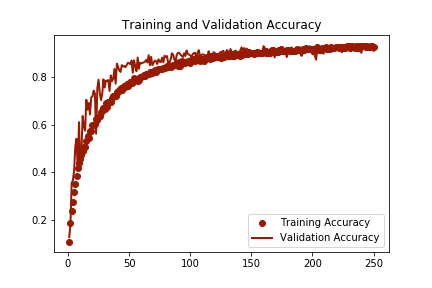
\includegraphics{train-vs-val-acc-medset4}
\newline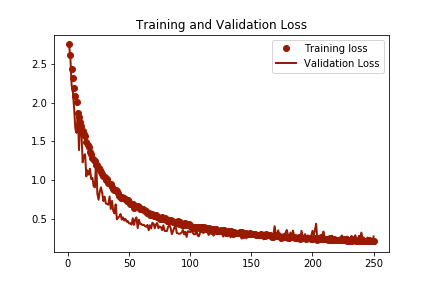
\includegraphics{train-vs-val-loss-medset4}
\item The following test, medset5, will continue the progress of 4. Primarily we will introduce batch normalization to the model.
\end{enumerate}

\subsection{July 5th, 2019}
\noindent\makebox[\linewidth]{\rule{15cm}{0.4pt}}
\begin{enumerate}[label = (\roman*)]
\item The gap in timing for updates has been due to the stall in model improvements over the last week.
\item As we continue to push forward in our efforts, we will most likely see that once we reach a certain point, the gains will take longer to achieve.
\item We are currently still on the medium test set, 19 images, and will continue to develop the model until we feel that our performance is as high as we would like. The work that is going on now is heavily tuning the hyper parameters of our most successful model so far. The hope is that by varying these parameters, we can find an optimal model for our next test which will involve a larger set of characters.
\item Most of these tests have yielded sporadic results. None of them were awful, but none of them yielded better results.
\item The following has been tried so far: Increasing dropout, decreasing batch size, adding batch normalization, adding convolution layers.
\item So far it seems like the road ahead will consist of doing this tuning for several weeks and seeing what we can get from it. I would estimate that if we can't get further than 93\% after a month or two then we will need to go back and gather more data, which very well may be necessary.
\item I am currently running the last training test of the day, and am hopeful that this will provide a useful direction to take the model.
\item The results are as follows:
\item 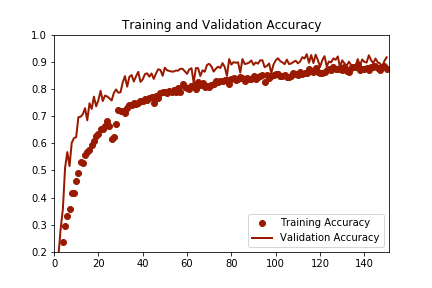
\includegraphics{acc_history5v4}
\item 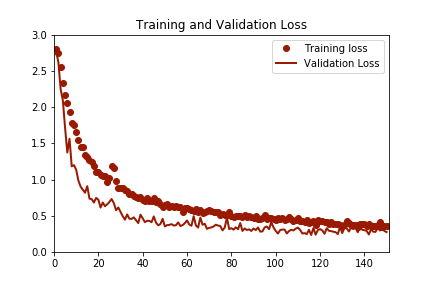
\includegraphics{loss_history5v4}
\item The results are preliminarily good, and I believe that we will be able to work to improve this version.
\end{enumerate}

\subsection{July 15th, 2019}
\noindent\makebox[\linewidth]{\rule{15cm}{0.4pt}}
\begin{enumerate}[label = (\roman*)]
\item After two weeks of rather stagnant improvements in test results, I decided to test a hypothesis.
\item It is my opinion that the training set for images in the first medium set may have been insufficient when given such large amounts of classes to choose from.
\item I posit that if I were to change the classes to those with more example data, the results of the training would improve dramatically. I have now started a medium set 2.0 test.
\item This test set will be 22 letters that have 8000 examples, compared to 5000 like the previous set of letters. This will give us a concrete decision of where to take our data set from here, more imaging seems necessary.
\item Today I have completed 4 tests that aim to get closer to this answer. From what I can ascertain, this network seems to be no better than the previous one. There is some improvement in overfitting, but the overall accuracy rate is not getting any higher. This obfuscates the original point of these tests, but I have 2 more that I think will give a better conclusion on this topic. 
\item There were some developments today that resulted in improvement over the previous 4 attempts today:
\item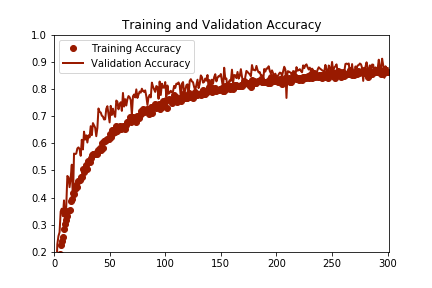
\includegraphics{acc_history5-20}
\item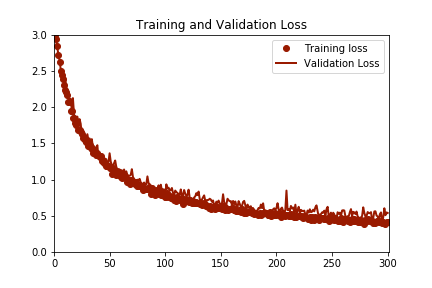
\includegraphics{loss_history5-20}
\item While these results are not our best they show that we may be suffering from a lack of data.
\item The final test is currently happening, this test uses our most successful large scale model so far, medset4 on a larger amount of data. 
\item The results from the final test will be present in tomorrow's update. The test will over run into tomorrow and will have to be paused.
\end{enumerate}

\subsection{July 16th, 2019}
\noindent\makebox[\linewidth]{\rule{15cm}{0.4pt}}
\begin{enumerate}[label = (\roman*)]
\item The truncated test from yesterday led to the following results:
\item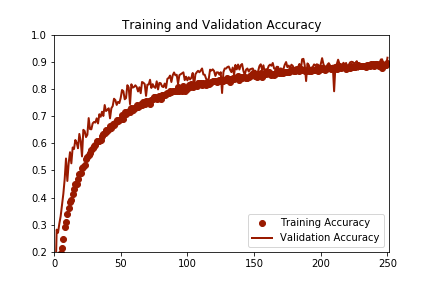
\includegraphics{{new_med_imgs/acc_history}}
\item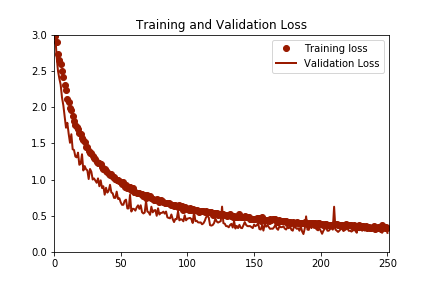
\includegraphics{{new_med_imgs/loss_history}}
\item The results are good, but still seem inconclusive. It does not appear clear that the lag in progress from previous iterations was due to a lack of data, although I think adding data would certainly improve scores.
\item In order to gauge the effect of increasing size relative to a single sample rather than a change in sample classes (as was done in the previous test), we chose to expand a data set through manual augmentation and comparing it to the same, unaugmented set.
\item We went back to the original smallset test, which has 4 classes with 1,539 images. Through a program called image transform  that I wrote, I augmented them and got 3,053 images total from the base set.
\item Examples of augmentation:
\item 
\includegraphics{{augmented/augmented_6}} 
\includegraphics{{augmented/augmented_61}} 
\includegraphics{{augmented/augmented_73}} 
\includegraphics{{augmented/augmented_87}}
\item The results were as follows:
\item Baseline:
\item 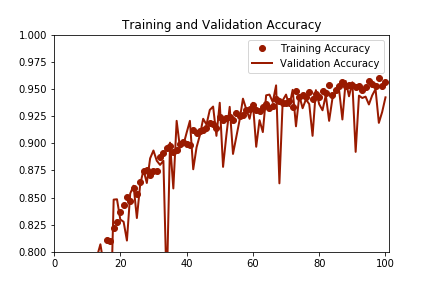
\includegraphics{{new_med_imgs/acc_historybaseline}}
\item 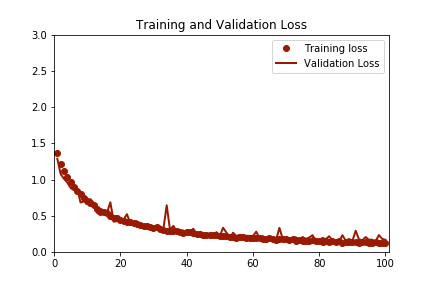
\includegraphics{{new_med_imgs/loss_historybaseline}}
\item Test:
\item 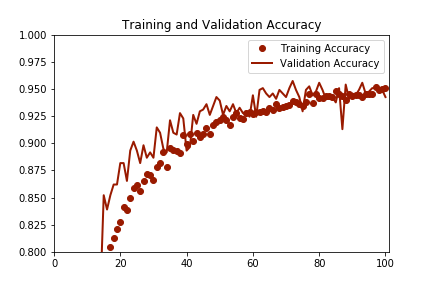
\includegraphics{{new_med_imgs/acc_historytest}}
\item 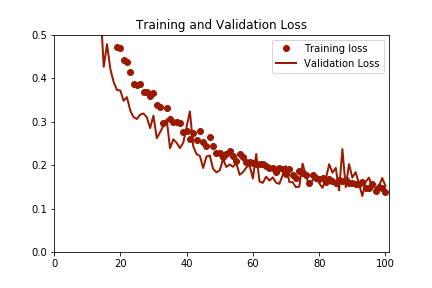
\includegraphics{{new_med_imgs/loss_historytest}}
\item The results are not significant, although the decrease in loss is notable. As can be seen in Figure XIV there appears to be a small uptick in accuracy at the end of the training cycle. We intend to test what happens with slightly increased training to 150 epochs.
\item Results:
\item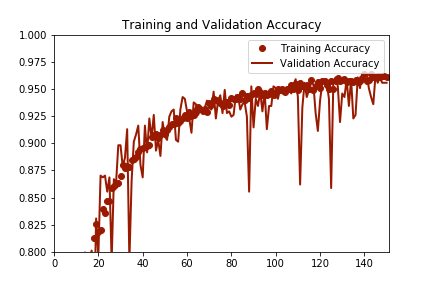
\includegraphics{{new_med_imgs/acc_historytest150epochs}}
\item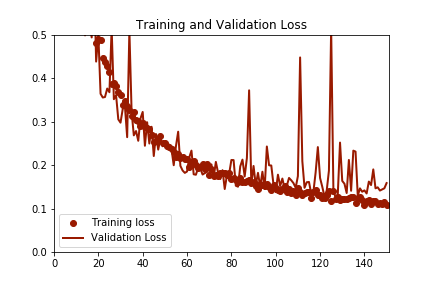
\includegraphics{{new_med_imgs/loss_historytest150epochs}}
\end{enumerate}


\subsection{July 17th, 2019}
\noindent\makebox[\linewidth]{\rule{15cm}{0.4pt}}
\begin{enumerate}[label = (\roman*)]
\item Yesterday I created a script that does large scale testing in order to compile data into csv files for visualization.
\item The script takes a path to the test files, a path to the model, and a dictionary of labels. The script then tests, and subsequently saves the results to a results.csv file.
\item This will be useful to document our results with.
\item There have been several important developments at the end of yesterday on the project. For one I rewrote the data manipulation script to be random and the results seem to be an increase of ~5\% over the previous version.
\item I have also modified the optimization function we use by adding an epsilon parameter of .9.
\item I have decided as well to increase dropout where possible to continue to limit our model's tendency to over fit. The results are great:
\item 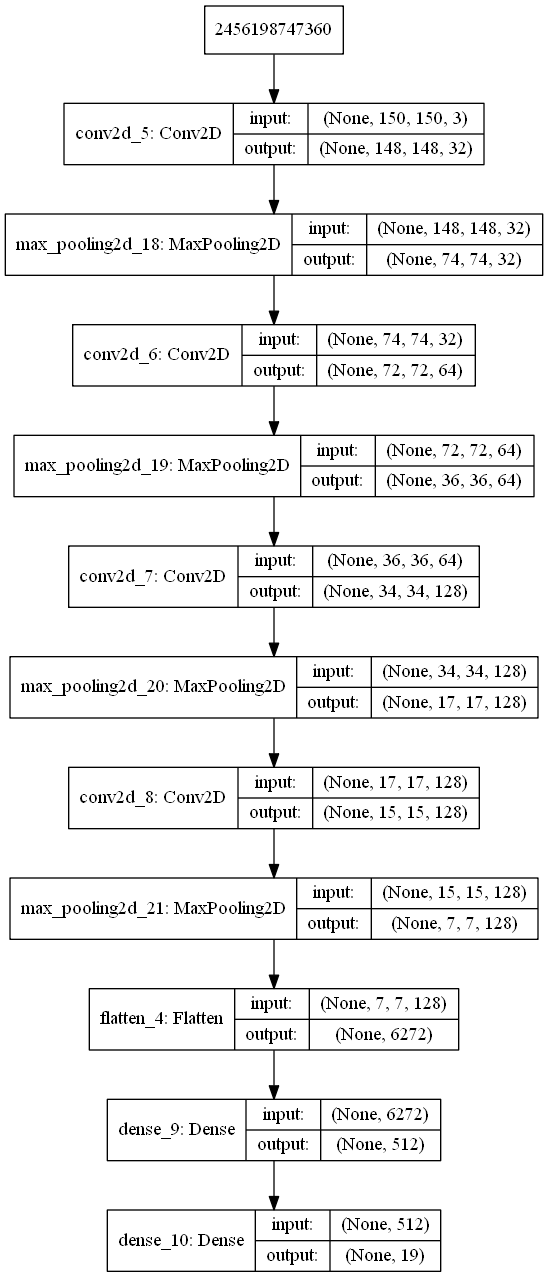
\includegraphics[height = 200mm, scale=.5]{{new_med_imgs/model}}
\item 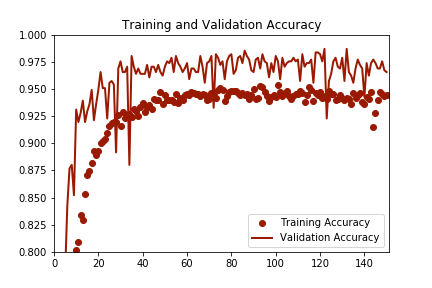
\includegraphics{{new_med_imgs/acc_historytest2}}
\item 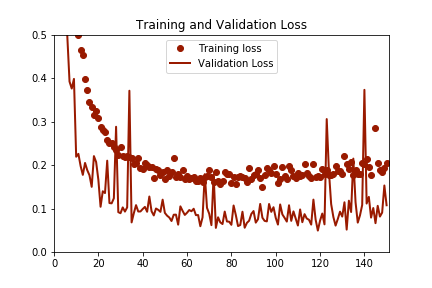
\includegraphics{new_med_imgs/loss_historytest2}
\item The small discrepancy between training and validation acc/loss is due to using dropout on the model, this difference would converge over time.
\end{enumerate}

\end{document}